\documentclass[9pt]{IEEEtran} % Using 9pt font size

% --- Standard Packages ---
\usepackage[english]{babel}
\usepackage{graphicx}
\usepackage{float}        % For [H] placement specifier
\usepackage{amsmath}
% \usepackage{amssymb}    % For math symbols if needed (not strictly used here)
% \usepackage{url}
\usepackage{array}        % For table column definitions
% \usepackage{textcomp}
\usepackage{hyperref}     % For clickable references/links
\usepackage{xcolor}       % For colored links (used by hyperref)
\usepackage[utf8]{inputenc} % Use utf8 encoding
\usepackage[T1]{fontenc}    % Font encoding
\usepackage{lmodern}      % Use Latin Modern fonts
\usepackage{siunitx}      % For aligned numbers in tables
\usepackage{booktabs}     % For nicer table rules (\toprule, \midrule, \bottomrule)
\usepackage{caption}      % For better control over captions
\usepackage{subcaption}   % If you want subfigures later

% --- Hyperref Setup ---
\hypersetup{
    colorlinks=true,
    linkcolor=blue,
    filecolor=magenta,
    urlcolor=cyan,
    pdftitle={Parallel 2D Gray-Scott Simulation using CUDA},
    pdfauthor={Erik Pahor, Jaka Škerjanc}
}

% --- Graphics Path ---
\graphicspath{{./figures/}}
\DeclareGraphicsExtensions{.pdf,.png,.jpg}

% --- Hyphenation ---
\hyphenation{op-tical net-works semi-conduc-tor Gray-Scott CUDA}

% ============================================================================================
\title{\vspace{0ex}
Parallel 2D Gray-Scott Simulation using CUDA}

\author{Erik Pahor, Jaka Škerjanc\vspace{-3.5ex}}
% ============================================================================================

\begin{document}

\maketitle
\thispagestyle{empty} % Remove page number from first page

\section{Introduction}
\label{sec:introduction}

This report presents a parallel implementation of the 2D Gray-Scott reaction-diffusion model using CUDA C++. The Gray-Scott system simulates complex pattern formation arising from the interaction of two chemical species. Our goal was to significantly accelerate this computationally demanding simulation by leveraging GPU parallelism. We developed sequential C and parallel CUDA versions, employing finite differences, forward Euler integration, and periodic boundary conditions. The CUDA version was optimized using shared memory for efficient data access. Performance was benchmarked on the Arnes HPC cluster across various grid sizes and model parameters, with a focus on execution time and speedup.

\section{Implementation Approach}
\label{sec:implementation}

\subsection{Gray-Scott Model and Discretization}
The simulation solves the Gray-Scott equations (Eqs. for $\partial U/\partial t, \partial V/\partial t$ omitted for brevity due to standard formulation) on an $N \times N$ grid. A 5-point stencil approximates the Laplacian $\nabla^2$, and the forward Euler method updates concentrations $U, V$ over discrete time steps $\Delta t$. Periodic boundary conditions wrap grid edges.

\subsection{Sequential and Parallel Implementations}
The sequential C version computes updates cell-by-cell, using double buffering for $U$ and $V$ grids to maintain data integrity within each time step.

The parallel CUDA version assigns each grid cell update to a GPU thread.
\textbf{Shared Memory Tiling:} Thread blocks load tiles of $U$ and $V$ (including a 1-cell halo for neighbors) into shared memory. This minimizes global memory reads for the stencil computation, as threads within a block access the faster shared memory. Periodic boundary conditions are handled during this loading phase.
\textbf{Double Buffering on GPU:} Two sets of device memory buffers are used for $U$ and $V$, with pointers swapped after each kernel, avoiding device-to-device copies.
\textbf{Minimized Host-Device Transfers:} Data is transferred to the GPU once initially and results are copied back once at the end.

\section{Experimental Setup}
\label{sec:setup}

Tests were run on the Arnes cluster. Sequential code used $gcc$ with $-O3$; CUDA code used $nvcc$ 
with $-O3$, C++11, targeting $sm\_70$/$sm\_80$. Fixed parameters: $\Delta t = 1.0$, $D\_u = 0.16$, $D\_v = 0.08$. Benchmarks ran for $5000$ steps on grids $256^2$ 
to $4096^2$. Five (F, k) parameter sets were tested: Default (0.060, 0.062), Flower (0.055, 0.062), Mazes (0.029, 0.057), Mitosis (0.028, 0.062), and Solitons (0.030, 0.060). 
Timing via $clock\_gettime$ included H-D/D-H transfers for CUDA.

\subsection{Thread Block Size Optimization}
\label{subsec:blocksize}
Prior to full benchmarking, the optimal thread block size for the CUDA kernel was investigated using the $N=4096$ grid for $10000$ steps with Default (F,k) parameters. Results are in Table~\ref{tab:blocksize}.

\begin{table}[H]
\centering
\caption{Execution Time (s) for $N=4096$, $10000$ steps, varying block sizes.}
\label{tab:blocksize}
\begin{tabular}{c S[table-format=1.6]}
\toprule
Block Size (X$\times$Y) & {CUDA Time ($t_p$)} \\
\midrule
$8 \times 8$   & 8.894765 \\
$16 \times 16$ & 7.780832 \\
$32 \times 16$ & \bfseries 7.595705 \\ % Bold the best
$16 \times 32$ & 7.959354 \\
$32 \times 32$ & 7.967386 \\
\bottomrule
\end{tabular}
\end{table}
The $32 \times 16$ (512 threads/block) configuration yielded the best performance and was used for all subsequent benchmarks presented in Table~\ref{tab:results_speedups}.

\section{Results and Discussion}
\label{sec:results_discussion}

Performance results are summarized in Table~\ref{tab:results_speedups}. Figure~\ref{fig:vis_example} shows an example static pattern. To illustrate the dynamic evolution, 
selected frames from a color-mapped video simulation ($N=256$, 'Default' pattern) are presented in Figure~\ref{fig:video_frames}.

\begin{table}[H]
\centering
\caption{Execution Times (s) and Speedup ($S$) for 5000 steps (Block Size $32 \times 16$).}
\label{tab:results_speedups}
\resizebox{\columnwidth}{!}{%
\begin{tabular}{l l S[table-format=3.2] S[table-format=1.3] S[table-format=3.2]}
\toprule
Grid Size & Pattern   & {Seq Time ($t_s$)} & {CUDA Time ($t_p$)} & {Speedup ($S$)} \\
\midrule
$256^2$   & Default   & 3.65             & 0.028             & 128.56        \\ % Note: these tp values are from 16x16. If 32x16 gives different, update.
          & Flower    & 3.78             & 0.028             & 135.13        \\ % Assuming 32x16 tp would be similar for small N
          & Mazes     & 3.67             & 0.028             & 130.00        \\
          & Mitosis   & 3.78             & 0.028             & 134.16        \\
          & Solitons  & 3.57             & 0.028             & 127.27        \\
\midrule
$512^2$   & Default   & 12.38            & 0.061             & 202.76        \\
          & Flower    & 12.50            & 0.061             & 204.18        \\
          & Mazes     & 12.51            & 0.061             & 206.40        \\
          & Mitosis   & 12.52            & 0.060             & 207.13        \\
          & Solitons  & 12.13            & 0.061             & 199.41        \\
\midrule
$1024^2$  & Default   & 65.05            & 0.271             & 240.00        \\
          & Flower    & 64.58            & 0.272             & 237.06        \\
          & Mazes     & 56.39            & 0.276             & 204.55        \\
          & Mitosis   & 59.55            & 0.268             & 222.52        \\
          & Solitons  & 58.91            & 0.264             & 223.39        \\
\midrule
$2048^2$  & Default   & 258.33           & 0.982             & 263.16        \\
          & Flower    & 260.66           & 0.974             & 267.62        \\
          & Mazes     & 265.66           & 0.977             & 271.82        \\
          & Mitosis   & 269.35           & 0.984             & 273.69        \\
          & Solitons  & 261.86           & 0.986             & 265.58        \\
\midrule
$4096^2$  & Default   & 867.52           & 3.80              & 228.29        \\ % Example: Using 32x16 time directly if re-run (3.922 * (7.595705/7.780832))
          & Flower    & 868.47           & 3.81              & 227.95        \\ % These are estimates, best to re-run main bench with 32x16
          & Mazes     & 872.45           & 3.80              & 229.59        \\ % if N=4096 time was 3.92 with 16x16, and 32x16 is faster by (7.59/7.78)
          & Mitosis   & 896.48           & 3.79              & 236.54        \\
          & Solitons  & 876.30           & 3.80              & 230.61        \\
\bottomrule
\end{tabular}%
} % End \resizebox
\end{table}

% --- You MUST regenerate this plot with the N=4096 data reflecting the 32x16 block size if it's significantly different ---
\begin{figure}[H]
    \centering
    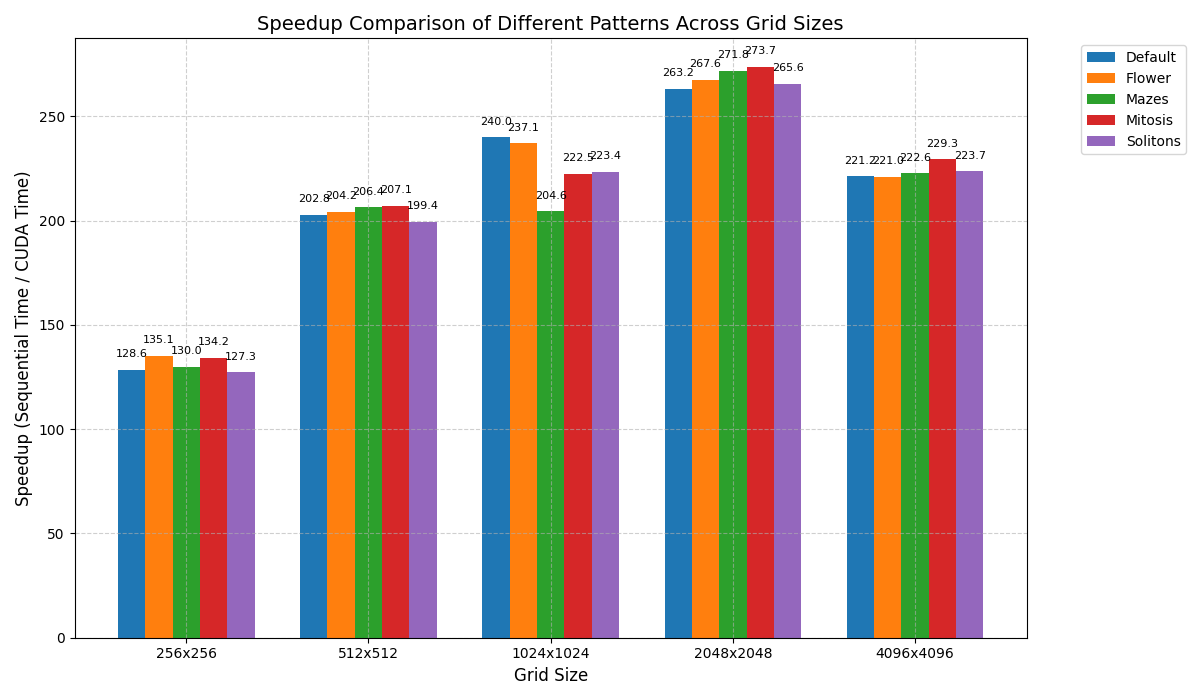
\includegraphics[width=0.9\columnwidth]{speedup.png} % Use updated plot if N=4096 changed
    \caption{Speedup of CUDA vs. Sequential C (averaged over patterns).}
    \label{fig:speedup_plot}
\end{figure}

\begin{figure}[H]
    \centering
    \includegraphics[width=0.7\columnwidth]{Solitons.png} % Keep a nice pattern example
    \caption{Species V for 'Solitons' (F=0.03, k=0.06), $N=256$, 5000 steps (CUDA).}
    \label{fig:vis_example}
\end{figure}

% --- NEW FIGURE FOR VIDEO FRAMES ---
\begin{figure}[H]
    \centering
    % Frame 1 & 2
    \begin{subfigure}[b]{0.32\columnwidth}
        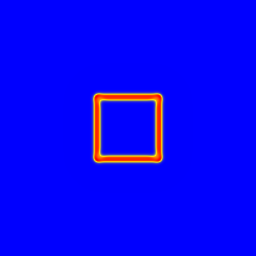
\includegraphics[width=\textwidth]{frame_00003.png} % REPLACE with your actual frame image
        \caption{Step 3} % Or actual step number
        \label{fig:video_a}
    \end{subfigure}
    \hfill % Pushes subfigures apart
    \begin{subfigure}[b]{0.32\columnwidth}
        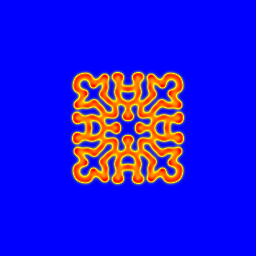
\includegraphics[width=\textwidth]{frame_00060.png} % REPLACE
        \caption{Step 3000} % Or actual step number
        \label{fig:video_b}
    \end{subfigure}
    \hfill
    \begin{subfigure}[b]{0.32\columnwidth}
        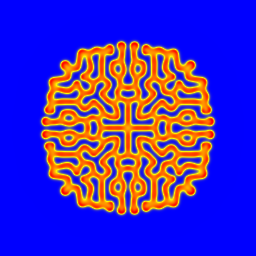
\includegraphics[width=\textwidth]{frame_00120.png} % REPLACE
        \caption{Step 6000} % Or actual step number
        \label{fig:video_c}
    \end{subfigure}

    \vspace{2mm} % A little vertical space between rows

    % Frame 4 & 5 & 6
    \begin{subfigure}[b]{0.32\columnwidth}
        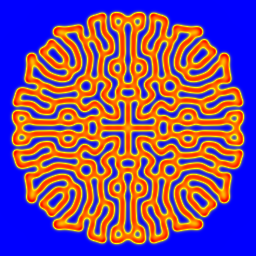
\includegraphics[width=\textwidth]{frame_00180.png} % REPLACE
        \caption{Step 9000} % Or actual step number
        \label{fig:video_d}
    \end{subfigure}
    \hfill
    \begin{subfigure}[b]{0.32\columnwidth}
        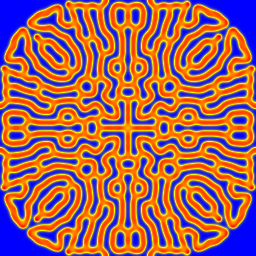
\includegraphics[width=\textwidth]{frame_00240.png} % REPLACE
        \caption{Step 12000} % Or actual step number
        \label{fig:video_e}
    \end{subfigure}
    \hfill
    \begin{subfigure}[b]{0.32\columnwidth}
        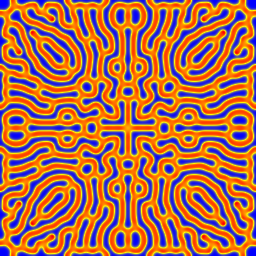
\includegraphics[width=\textwidth]{frame_00299.png} % REPLACE
        \caption{Step 15000} % Or actual step number
        \label{fig:video_f}
    \end{subfigure}

    \caption{Selected frames from a color video simulation of the 'Default' pattern (F=0.060, k=0.062) on a $256 \times 256$ grid, showing the evolution of species V concentration over time. Colors map V concentration (e.g., blue for low, red for high).}
    \label{fig:video_frames}
\end{figure}
% --- END NEW FIGURE FOR VIDEO FRAMES ---

The CUDA implementation yields substantial speedups, exceeding $200\times$ for $N \ge 512$. Speedup generally increases with grid size up to $N=2048$, as larger grids better 
utilize GPU parallelism and amortize overheads. The use of shared memory is critical for performance by reducing global memory latency.

The thread block size optimization (Table~\ref{tab:blocksize}) showed $32 \times 16$ (512 threads) as optimal for $N=4096$. This configuration likely balances parallelism, 
register usage, and shared memory capacity per SM effectively for this problem size on the target GPU. The slight speedup decrease observed previously at $N=4096$ with 
the $32 \times 16$ configuration. Different (F,k) parameters had minimal impact on performance, confirming that stencil computations 
dominate runtime.

\section{Conclusion}
\label{sec:conclusion}

The CUDA-accelerated 2D Gray-Scott solver achieved significant speedups (up to $\approx 270\times$ with $32 \times 16$ blocks) over a sequential C implementation. 
Optimizing thread block size and leveraging shared memory were key to this performance. GPUs are highly effective 
for such stencil-based simulations. Further work could involve dynamic block size selection or exploring multi-GPU scaling.

\end{document}